\chapter{Architektura systemu}
\label{sec:piaty}
\section{Podział na projekty Eclipse}

Opracowany system opiera się na architekturze platformy \emph{Eclipse}, która pozwala na rozszerzanie jej funkcjonalności na podstawie ściśle określonej struktury. Struktura ta opisuje poszczególne moduły, jakie mogą znaleźć się w tworzonej wtyczce (np. widoki, edytory, obsługa zewnętrznych narzędzi) oraz sposób ich współpracy z pozostałą częścią programu. Aby dodać niedostępną standardowo funkcję, wystarczy rozszerzyć odpowiedni moduł, wykorzystując przy tym zdefiniowane klasy i interfejsy. Taka budowa powoduje, że większość wtyczek posiada takie same elementy składowe, będące w większości własną implementacją standardowych komponentów \emph{Eclipse}.

W przypadku systemu GUI4PDDL są to:
\begin{itemize}
\item Edytor kodu wraz z analizatorem kodu i podpowiadaniem składni.
\item Widoki preferencji wtyczki oraz przeglądarki planów.
\item Obsługa uruchamiania zewnętrznych narzędzi (planerów).
\item Kreatory nowego projektu i pliku PDDL.
\end{itemize}

Ze względu na złożoność oraz zakres wymagań projekt GUI4PDDL podzielono na 6~głównych podprojektów związanych z rozwojem wtyczki oraz 2 dodatkowe, standardowe projekty \emph{Eclipse}, służące do testowania istniejących rozwiązań. Taka struktura pozwala na logiczne oddzielenie implementacji wtyczki od kodu, odpowiedzialnego za jej testowanie i integrację z \emph{Eclipse}. Pozwala to zmniejszyć rozmiar plików pobieranych przy instalacji przez użytkownika, zwłaszcza dodatkowych bibliotek.

Zgodnie z konwencją nazewniczą pakietów języka Java, wszystkie główne projekty mają przedrostek \texttt{pl.poznan.put.cs.gui4pddl}, natomiast w pozostałych obowiązują dowolne nazwy. Dokładna struktura i opis poszczególnych projektów przedstawiono poniżej.

Projekty główne:
\begin{description}
\item [\texttt{pl.poznan.put.cs.gui4pddl}] Projekt zawierający pełną implementację wtyczki (wersję instalacyjną). Składa się z pakietów odpowiedzialnych za logikę biznesową oraz wszystkie istniejące widoki. Szerszy opis tego projektu znajduje się w rozdziale~\ref{sec:struktura}.
\item [\texttt{pl.poznan.put.cs.gui4pddl.antlr}] Projekt zawierający bibliotekę \emph{ANTLR Runtime}, niezbędną do działania analizatora składniowego PDDL, wykonanego w narzędziu \emph{ANTLR}\footnote{\url{http://www.antlr.org/}}.
\begin{sloppypar}
\item [\texttt{pl.poznan.put.cs.gui4pddl.feature}] Projekt \emph{Feature}\footnote{\url{http://help.eclipse.org/juno/topic/org.eclipse.pde.doc.user/concepts/feature.htm?cp=4_1_1}}, umożliwiający połączenie różnych wtyczek w taki sposób, by z zewnątrz były traktowane jako logiczna całość, co ułatwia zarządzanie nimi. Dodatkowo pozwala na uzupełnienie informacji dotyczących wersji, licencji, obsługiwanych systemów operacyjnych itp. Projekt tego typu wymagany jest także w procesie budowania i aktualizacji. Wykorzystany w niniejszej pracy, grupuje podprojekty \texttt{pl.poznan.put.cs.gui4pddl} oraz \texttt{pl.poznan.put.cs.gui4pddl.antlr}, a także udostępnia podstawowe informacje o narzędziu GUI4PDDL.
\end{sloppypar}
\item [\texttt{pl.poznan.put.cs.gui4pddl.tests}] Projekt zawierający testy jednostkowe kodu niezwiązanego z interfejsem graficznym, wykorzystujące bibliotekę \emph{JUnit}\footnote{\url{http://junit.org/}} oraz testy gramatyki formalnej, generowanej przez narzędzie \emph{ANTLR}, wykorzystujące bibliotekę \emph{gUnit}\footnote{\url{http://www.antlr.org/wiki/display/ANTLR3/gUnit+-+Grammar+Unit+Testing}}.  Oddzielenie testów od kodu głównego projektu pozwoliło na zmniejszenie wielkości wersji instalacyjnej oraz zredukowanie zależności od dodatkowych bibliotek.
\item [\texttt{pl.poznan.put.cs.gui4pddl.uitests}] Projekt zawierający testy jednostkowe interfejsu graficznego, wykorzystujące bibliotekę \emph{SWTBot}\footnote{\url{http://eclipse.org/swtbot/}}. Biblioteka ta umożliwia przeprowadzenie automatycznych testów akceptacyjnych GUI, stworzonego przy pomocy biblioteki \emph{SWT}\footnote{\url{http://eclipse.org/swt/}}.
\item [\texttt{pl.poznan.put.cs.gui4pddl.update}] Projekt typu \emph{Update site}\footnote{\url{http://help.eclipse.org/juno/topic/org.eclipse.pde.doc.user/concepts/update_site.htm?cp=4_1_6}}, zawierający statyczne pliki, które mogą być umieszczone w określonym miejscu na serwerze. Użytkownicy, korzystając z adresu do tego miejsca mogą pobrać i zainstalować wtyczkę poprzez menedżer aktualizacji. Projekt ten korzysta z wcześniej zdefiniowanego projektu \emph{Feature} oraz zawiera opis wtyczki i kategorię, wyświetlone następnie przy instalacji.
\end{description}

Pozostałe projekty:
\begin{description}
\item [\texttt{RubikCube}] Przykładowy projekt PDDL wykorzystywany podczas rozwijania wtyczki. Zawiera zadanie automatycznego planowania, które z racji swojego charakteru oraz używanego planera wykonywało się przez znaczny czas, co było pomocne podczas testowania przerywania procesu planowania (roz. \ref{subsec:przerywanie}).
\item [\texttt{WorldOfBlocks}] Przykładowy projekt PDDL wykorzystywany podczas rozwijania wtyczki. Zawiera zadanie automatycznego planowania, które z racji swojego charakteru oraz używanego planera wykonywało się przez krótki czas.
\end{description}

\section{Struktura wtyczki}
\label{sec:struktura}

Kod głównego projektu wtyczki GUI4PDDL (\texttt{pl.poznan.put.cs.gui4pddl}) podzielony jest pomiędzy szereg pakietów, których nazwy, zgodnie z konwencją przyjętą w języku Java wskazują na zakres odpowiedzialności. Struktura projektu przedstawiona jest na rysunku~\ref{fig:packets_scheme}. Wyróżnić można kilka odrębnych grup oraz podpakiety.

\begin{figure}[h!]
    \centering
    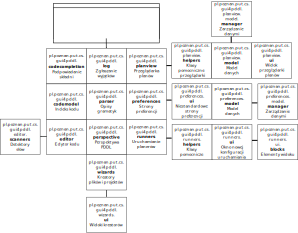
\includegraphics[width=\textwidth]{img/packets_scheme}
    \caption{Struktura pakietów. Strzałki wskazują na elementy znajdujące się na niższym poziomie w hierarchii pakietów.}
    \label{fig:packets_scheme}
\end{figure}

\begin{description}
\item [\texttt{pl.poznan.put.cs.gui4pddl}] Podstawowy pakiet projektu, zawierający implementację (klasa \texttt{Activator}) klasy \texttt{Plugin}, którą musi implementować każda wtyczka platformy \emph{Eclipse}. Klasa ta odpowiada za cykl życia (inicjalizacja, zakończenie) projektu. W~pakiecie tym znajdują się również współdzielone stałe oraz klasy pomocnicze, służące do tworzenia nowego projektu i przechowywania obrazów, wykorzystywanych we wtyczce.
\item [\texttt{pl.poznan.put.cs.gui4pddl.codecompletion}] Pakiet zawierający klasy odpowiedzialne za zarządzanie podpowiadaniem składni, w tym za tworzenie prawidłowych propozycji uzupełniania kodu.
\item [\texttt{pl.poznan.put.cs.gui4pddl.codemodel}] Pakiet zawierający klasy wchodzące w skład indeksu kodu (roz~\ref{subsec:indeks}), czyli modelu struktur PDDL. Znajdują się tam klasy reprezentujące m.in. akcje, predykaty, problemy i dziedziny.
\item [\texttt{pl.poznan.put.cs.gui4pddl.editor}] Pakiet zawierający implementację edytora tekstowego oraz wszystkich jego funkcji: kolorowania i podpowiadania składni, dopasowywania nawiasów, automatycznych wcięć.
\begin{itemize}
\item \texttt{\textbf{pl.poznan.put.cs.gui4pddl.editor.scanners}} Pakiet zawierający detektory słów kluczowych oraz elementów składniowych języka, które są wykorzystywane na etapie kolorowania i podpowiadania składni.
\end{itemize}
\item [\texttt{pl.poznan.put.cs.gui4pddl.log}] Pakiet zawierający klasę \texttt{Log}, wykorzystywaną jako mechanizm prostego zgłaszania wyjątków w czasie działania wtyczki. Wyjątki te są widoczne w widoku \textit{Error Log} platformy Eclipse.
\item [\texttt{pl.poznan.put.cs.gui4pddl.parser}] Pakiet zawierający pliki z opisami gramatyk, wykorzystanych do budowy analizatora kodu PDDL oraz klasy pomocnicze.
\item [\texttt{pl.poznan.put.cs.gui4pddl.perspective}] Pakiet zawierający definicję perspektywy\footnote{\url{http://help.eclipse.org/juno/topic/org.eclipse.platform.doc.user/concepts/concepts-4.htm?cp=0_2_2}} PDDL, czyli widocznego układu widoków podczas edycji plików PDDL. Charakterystycznymi elementami tej perspektywy są: przeglądarka projektów (ang. \textit{Project Explorer}), edytor plików oraz przeglądarka planów (ang. \textit{Plan Browser}, opis znajdue się w~rozdziale \ref{subsec:uruchamianie}).
\item [\texttt{pl.poznan.put.cs.gui4pddl.planview}] Pakiet związany z implementacją przeglądarki planów.
\begin{itemize}
\item \texttt{\textbf{pl.poznan.put.cs.gui4pddl.planview.helpers}} Pakiet zawierający klasy pomocnicze, służące do wyświetlania planów w zewnętrznym edytorze oraz uruchamiania systemowej przeglądarki plików, a także przetwarzania wzorca regularnego nazwy planu, zdefiniowanego w preferencjach planera (roz.~\ref{subsec:konfiguracja}).
\item \texttt{\textbf{pl.poznan.put.cs.gui4pddl.planview.model}} Pakiet zawierający klasę modelu danych, wykorzystywaną w przeglądarce planów.
\begin{itemize}
\item \texttt{\textbf{pl.poznan.put.cs.gui4pddl.planview.model.manager}} Pakiet zawierający klasy zarządzające danymi przeglądarki planów. Umożliwiają zapisanie oraz wczytywanie danych z~pliku XML oraz dodawanie i usuwanie elementów z~jednoczesną aktualizacją widoku przeglądarki.
\end{itemize}
\item \texttt{\textbf{pl.poznan.put.cs.gui4pddl.planview.ui}} Pakiet zawierający pełną implementację widoku przeglądarki planów.
\end{itemize}
\item \texttt{\textbf{pl.poznan.put.cs.gui4pddl.preferences}} Pakiet zawierający implementację widoków standardowych stron preferencji wtyczki, tzn. takich, które korzystają z API \emph{Preferences}\footnote{\url{http://help.eclipse.org/kepler/topic/org.eclipse.platform.doc.isv/guide/preferences_prefs.htm?cp=2_0_4_3}}. Są to preferencje ogólne, edytora oraz planera, dostępne z menu głównego \textit{Window} pod elementem \textit{Preferences}.
\begin{itemize}
\item \texttt{\textbf{pl.poznan.put.cs.gui4pddl.preferences.model}} Pakiet zawierający klasę modelu danych preferencji planera.
\begin{itemize}
\item \texttt{\textbf{pl.poznan.put.cs.gui4pddl.preferences.model.manager}} Pakiet zawierający klasę zarządzającą danymi preferencji planera. Pozwala na zapis i odczyt danych z pliku w formacie XML.
\end{itemize}
\item \texttt{\textbf{pl.poznan.put.cs.gui4pddl.preferences.ui}} Pakiet zawierający implementację niestandardowych widoków preferencji, tzn. takich, które nie korzystają z API \emph{Preferences} -- widok preferencji planera oraz jego okna dialogowe.
\end{itemize}
\item [\texttt{pl.poznan.put.cs.gui4pddl.runners}] Pakiet zawierający klasy odpowiedzialne za wywołanie planera (roz.~\ref{subsec:uruchamianie}), od momentu wciśnięcia przycisku \textit{Run}, poprzez stworzenie nowej konfiguracji uruchamiania, aż do inicjalizacji procesu zewnętrznego narzędzia. W pakiecie tym znajduje się także implementacja przerywania procesu znajdowania planu opisana w rozdziale~\ref{subsec:przerywanie}.
\begin{itemize}
\item \texttt{\textbf{pl.poznan.put.cs.gui4pddl.runners.helpers}} Pakiet zawierający pomocniczą kla\-sę metod, wykorzystywanych podczas uruchamiania planera. Funkcje te odpowiadają m.in. za przetwarzanie ścieżek do plików projektu oraz tworzenie drzewa katalogów dla wyników procesu planowania.
\item \texttt{\textbf{pl.poznan.put.cs.gui4pddl.runners.ui}} Pakiet zawierający klasy, związane z~tworzeniem okna nowej konfiguracji uruchamiania, dostępnego podczas inicjalizacji zewnętrznego narzędzia lub poprzez wybranie z menu \textit{Run} elementu \textit{Run Configurations...} i przejście na zakładkę \textit{PDDL}.
\begin{itemize}
\item \texttt{\textbf{pl.poznan.put.cs.gui4pddl.runners.ui.blocks}} Pakiet zawierający klasy odpowiedzialne za elementy widoku okna nowej konfiguracji uruchamiania.
\end{itemize}
\end{itemize}
\item [\texttt{pl.poznan.put.cs.gui4pddl.wizards}] Pakiet związany z implementacją dostępnych we wty\-czce kreatorów.
\begin{itemize}
\item \texttt{\textbf{pl.poznan.put.cs.gui4pddl.wizards.ui}} Pakiet zawierający implementację kreatorów tworzenia nowego projektu PDDL oraz nowego pliku dziedziny lub problemu.
\end{itemize}
\end{description}
